\documentclass{article}
\usepackage[utf8]{inputenc}
\usepackage{graphicx}
\usepackage{amsmath }
\usepackage{amssymb}
\usepackage{subcaption}
\usepackage{float}
\usepackage{mathtools}
\usepackage{algorithm}
\usepackage{algorithmic}
\usepackage{multirow}
\setcounter{section}{0}


\usepackage{cleveref} %referencing figures, equations and tables
\crefformat{figure}{Figure.~#2#1#3}
\crefformat{equation}{Eq.~#2#1#3}
\crefformat{table}{Table.~#2#1#3}
\crefformat{appendix}{Appendix.~#2#1#3}
\crefformat{section}{Section.~#2#1#3}

\title{Lagrange Multiplier and Penalty Method in Contact Mechanics}
\author{Amir Baharvand }
\date{}

\begin{document}

\maketitle

\section{Problem Statement}
 A cantilever beam with a Young's modulus 210GPa and yeilding stress 200MPa, shown in \cref{fig:beam}, undergoes a point load, $F$=565486.67N, at its middle point in the $x$-direction. A rigid wall is located at a distance of 0.1mm in the positive direction of the $x$-axis. To solve the problem using the finite element method, the beam is divided into four elements as illustrated in \cref{fig:tapered_beam}. The numerical model consists of four bar elements with only one degree of freedom in the $x$-direction as shown in \cref{fig:beam_fem}. The problem can be summarized as 
 
 \begin{equation}
     \begin{aligned}
    \min \quad & \Pi\\
    \textrm{s.t.} \quad & u_5 - 0.1\text{e-3} = 0\\
    \end{aligned}
    \label{eq:problem}
\end{equation}

where $\Pi$ is the potential energy and $u_5$ indicates the displacement of node 5 (see \cref{fig:beam_fem}). $\Pi$ is the difference between the strain energy and work done by external forces and can be written in the following matrix form.

\begin{equation}
    \Pi = \dfrac{1}{2} \mathbf{D}^{T} \mathbf{K} \mathbf{D} -  \mathbf{D}^{T}  \mathbf{P}
    \label{eq:potential_energy}
\end{equation}

$\mathbf{D}$ is the displacement, $\mathbf{K}$ is the tangential stiffness matrix, $\mathbf{P}$ is the external load and the superscript $T$ indicates the transpose. In the following, we solve the problem using the Lagrange multipliers and penalty methods. In penalty method, we also investigate the inherited penetration into the rigid wall due to the algorithm implementation. 
 
\begin{figure}[ht]
    \centering
        \begin{subfigure}{0.49\textwidth}
            \includegraphics[width=1\linewidth]{figures/beam.pdf} 
            \caption{}
            \label{fig:beam}
        \end{subfigure}
        \begin{subfigure}{0.49\textwidth}
            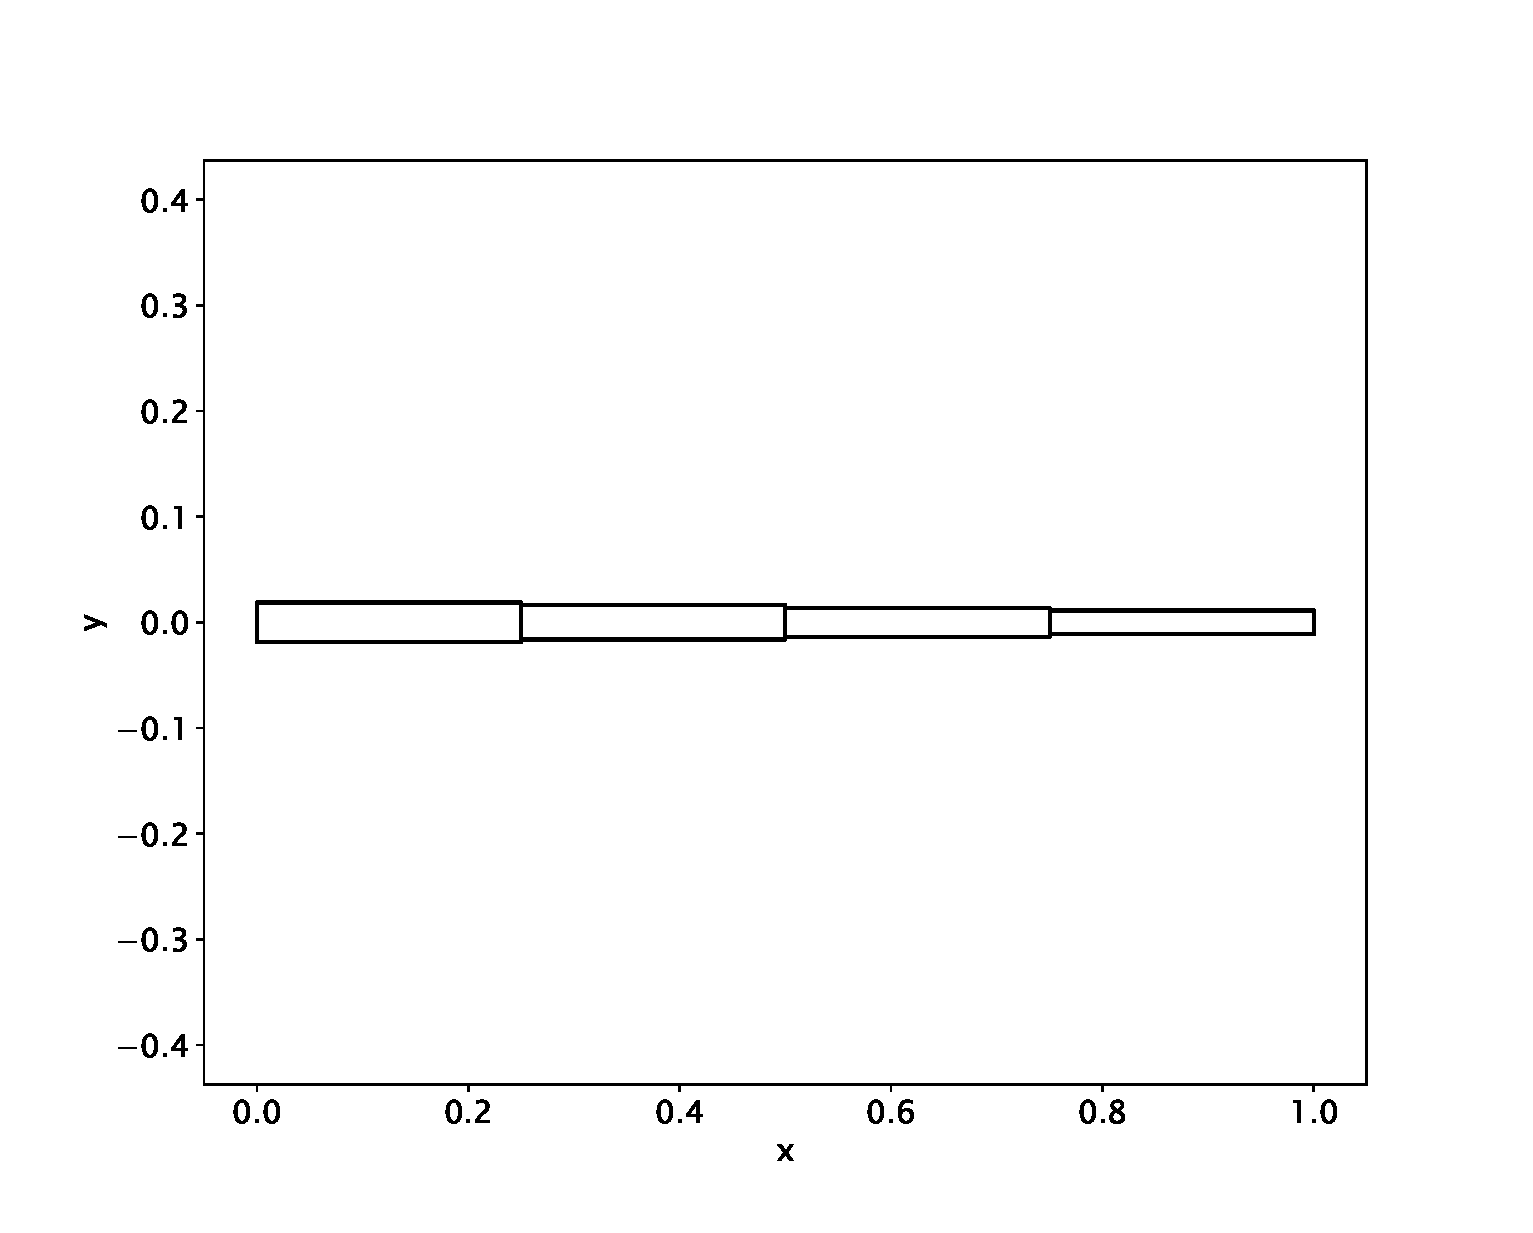
\includegraphics[width=1\linewidth]{figures/tapered_beam.eps} 
            \caption{}
            \label{fig:tapered_beam}
        \end{subfigure}
        \begin{subfigure}{0.49\textwidth}
            \includegraphics[width=1\linewidth]{figures/beam_fem.pdf} 
            \caption{}
            \label{fig:beam_fem}
        \end{subfigure}
    \caption{(a) The cantilever tapered beam. (b) The beam model with four elements. (c) The numerical model of the beam with bar elements.}
    \label{fig:beam_problem}
\end{figure}

\section{Lagrange Multiplier}
To impose the constraint given in \cref{eq:problem} using the Lagrange multiplier, we add a vector of Lagrange multipliers, $\mathbf{\lambda}$ to \cref{eq:potential_energy} and solve the minimization problem by taking the derivative of the potential energy w.r.t the displacement ($\partial \Pi / \partial \mathbf{D}$) and Lagrange multipliers ($\partial \Pi / \partial \mathbf{\lambda}$). As a result, \cref{eq:potential_energy} becomes \cite{cook2001}

\begin{equation}
    \Pi = \dfrac{1}{2} \mathbf{D}^{T} \mathbf{K} \mathbf{D} -  \mathbf{D}^{T}  \mathbf{P} + \lambda^{T} ( \mathbf{C} \mathbf{D} -  \mathbf{F})
    \label{eq:lm}
\end{equation}

where $\lambda$ is the Lagrange multiplier, $\mathbf{C}$ is the constraint (the coefficient of $u_5$ in \cref{eq:problem}) and $\mathbf{F}$ is the constraint value (0.1e-3 in \cref{eq:problem}). After taking the derivatives, the final equation can be written in the following matrix form \cite{cook2001}.

\begin{equation*}
    \begin{bmatrix}
\mathbf{K} & \mathbf{C}^{T} \\ 
\mathbf{C} & 0
\end{bmatrix}
\begin{Bmatrix}
\mathbf{D}\\ 
\mathbf{\lambda}
\end{Bmatrix} = 
\begin{Bmatrix}
\mathbf{P}\\ 
\mathbf{F}
\end{Bmatrix}
\end{equation*}

A Python script is developed based on \cref{alg:lm}. 

\begin{algorithm}[H]
\caption{Lagrange multiplier pseudocode.}
\begin{algorithmic} 
\ENSURE $D = 0, K = 0$
\STATE Compute $K$
\STATE $K$ $\leftarrow$ Assemble $K$ and $C$
\STATE Apply B.C on $K$
\STATE $P$ $\leftarrow$ Assemble $P$ and $F$
\STATE Solve $D = K^{-1} P$
\end{algorithmic}
\label{alg:lm}
\end{algorithm}

\cref{fig:lm} shows the undeformed and deformed configuration of the beam using the Lagrange multiplier method. As it is clearly visible the Lagrange multiplier solution is exact and the beam does not penetrate in the rigid wall. 

\begin{figure}[H]
    \centering
    \includegraphics[width = 0.8\textwidth ]{figures/lm.png}
    \caption{The undeformed and deformed state of the beam using the Lagrange multiplier method.}
    \label{fig:lm}
\end{figure}

\section{Penalty Method}
Unlike the Lagrange multiplier, the penalty method does not introduce any extra variable; however, the accuracy of the solution depends on the penalty coefficient in this method. Therefore, \cref{eq:potential_energy} remains intact while the values of $\mathbf{K}$ and $\mathbf{P}$ are manipulated using the penalty coefficient, $\epsilon_p$. \cref{alg:pm} summarizes the penalty method implementation.


\begin{algorithm}[H]
\caption{Penalty method pseudocode.}
\begin{algorithmic} 
\ENSURE $D = 0, K = 0, \epsilon_p = 1e14$
\STATE Compute $K$
\STATE $K$ $\leftarrow$ $K + \epsilon_p C^{T} C$
\STATE Apply B.C on $K$
\STATE $P$ $\leftarrow$ $P + \epsilon_p F$
\STATE Solve $D = K^{-1} P$
\end{algorithmic}
\label{alg:pm}
\end{algorithm}

\cref{fig:pm_study} shows the effect of $\epsilon_p$ on the accuracy of the solution using the penalty method. It is seen that by increasing $\epsilon_p$, the solution converges 0.1mm.

\begin{figure}[H]
    \centering
    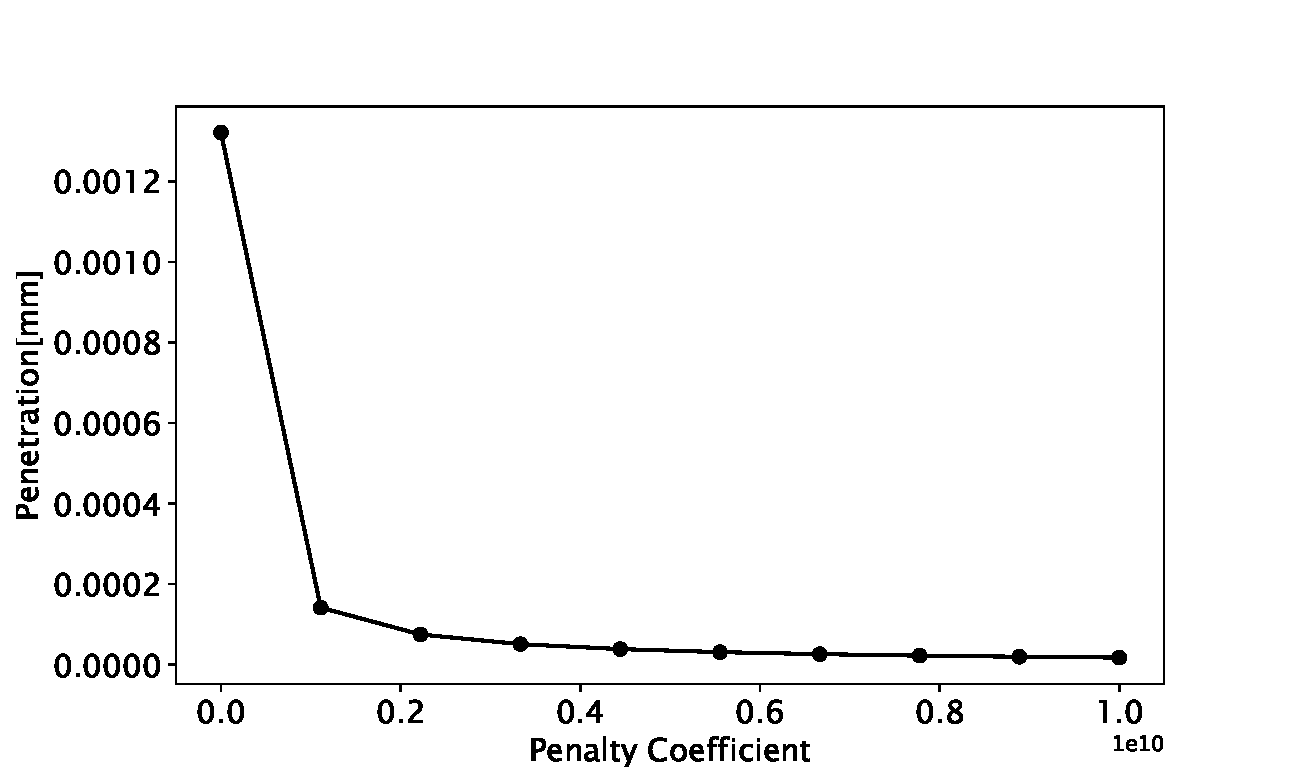
\includegraphics[width = 0.7\textwidth ]{figures/penalty.eps}
    \caption{The effect of penalty coefficient on the accuracy of the solution.}
    \label{fig:pm_study}
\end{figure}

\cref{tab:pm} shows the penetration values for various $\epsilon_p$. The penetration vanishes at about $\epsilon_p$ = 1e14. 

\begin{table}[H]
    \centering
    \caption{Penalty coefficients and their corresponding penetration values in penalty method.}
    \begin{tabular}{cc} \hline
    $\epsilon_p$ & Penetration[mm] \\ \hline
        1 & 1.32e-03 \\
        1e5 & 1.32e-03 \\
        1e6 & 1.31e-03 \\
        1e7 & 1.23e-03 \\
        1e8 & 7.54e-04 \\
        1e9 & 1.55e-04 \\
        1e10 & 1.73e-05\\
        1e11 & 1.76e-06\\
        1e12 & 1.76e-07\\
        1e13 & 1.76e-08\\
        1e14 & 1.79e-09\\ \hline
    \end{tabular}
    \label{tab:pm}
\end{table}

\cref{fig:pm1} (maximum penetration) and \cref{fig:pm1e14} (no penetration) shows the penetration into the rigid body.

\begin{figure}[ht]
    \centering
        \begin{subfigure}{0.49\textwidth}
            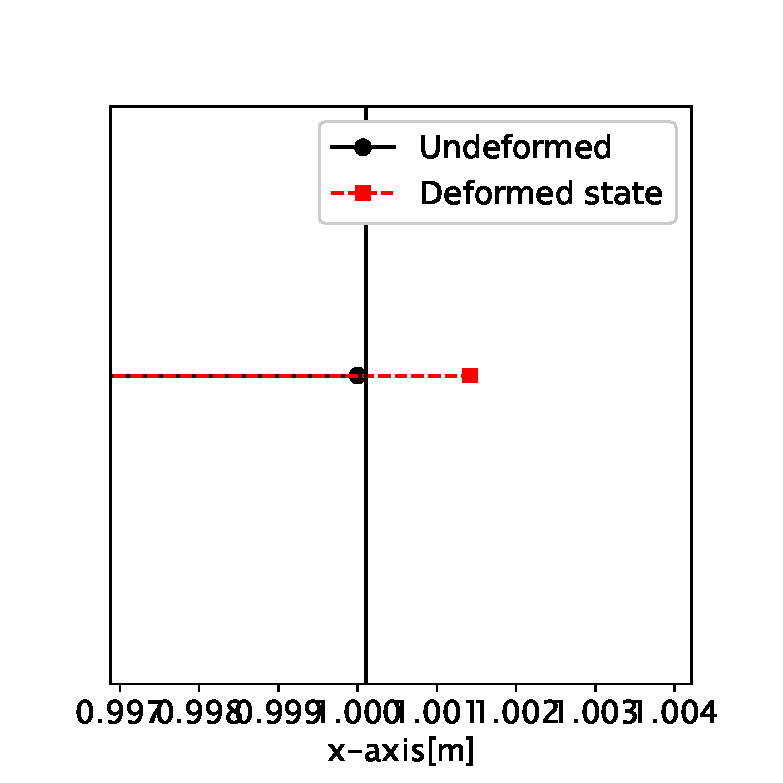
\includegraphics[width=1\linewidth]{figures/pm1.eps} 
            \caption{$\epsilon_p$=1}
            \label{fig:pm1}
        \end{subfigure}
        \begin{subfigure}{0.49\textwidth}
            \includegraphics[width=1\linewidth]{figures/pm1e14.eps} 
            \caption{$\epsilon_p$=1e14}
            \label{fig:pm1e14}
        \end{subfigure}
    \caption{The penetration of beam into the rigid wall in the penalty method.}
    % \label{}
\end{figure}


\newpage
\bibliography{ref}
\bibliographystyle{ieeetr}

\end{document}